% Adiciona workflow para compilar LaTeX para PDF
% https://chatgpt.com/share/68016842-23b8-8008-bafb-2084e351a35c

% SVG
% pdflatex --shell-escape arquivo.tex

% PlantUML
% https://chatgpt.com/share/68018f2e-9cf4-8008-b2e2-87a70beddf46

\documentclass[12pt]{article}

\usepackage{sbc-template}
\usepackage{graphicx,url}
\usepackage[utf8]{inputenc}
\usepackage[brazil]{babel}
\usepackage{svg}
% \usepackage{plantuml}
\usepackage{float}

\sloppy

\title{Título do Artigo:\\ Subtítulo do artigo}

\author{Dalton Solano dos Reis\inst{1}, % Luciana P. de A. Kohler \inst{1}, 
    Marcelo da Silva Hounsell\inst{2} }

\address{Departamento de Sistemas e Computação\\ Universidade Regional de Blumenal (FURB) -- Blumenau, SC -- Brazil
\nextinstitute
  Centro de Ciências Tecnológicas\\ Universidade do Estado de Santa Catarina (UDESC) -- Joinville, SC -- Brazil
\email{\{dalton,Lpa\}@furb.br, marcelo.hounsell@udesc.br}
}

\begin{document} 

\maketitle

\begin{abstract}
  This meta-paper describes the style to be used in articles and short papers for SBC conferences. For papers in English, you should add just an abstract while for the papers in Portuguese, we also ask for an abstract in Portuguese (``resumo''). In both cases, abstracts should not have more than 10 lines and must be in the first page of the paper.
\end{abstract}
     
\begin{resumo} 
  Este meta-artigo descreve o estilo a ser usado na confecção de artigos e resumos de artigos para publicação nos anais das conferências organizadas pela SBC. É solicitada a escrita de resumo e abstract apenas para os artigos escritos em português. Artigos em inglês deverão apresentar apenas abstract. Nos dois casos, o autor deve tomar cuidado para que o resumo (e o abstract) não ultrapassem 10 linhas cada, sendo que ambos devem estar na primeira página do artigo.
\end{resumo}

\section{Informações Gerais}

Todos os artigos completos e pôsteres (artigos curtos) submetidos a algum congresso da SBC, incluindo quaisquer documentos de apoio, devem ser redigidos em inglês ou em português. O formato do artigo deve ser A4, com uma única coluna, margem superior de 3,5 cm, inferior de 2,5 cm e margens laterais de 3,0 cm, sem cabeçalhos ou rodapés. A fonte principal deve ser Times, tamanho nominal 12, com espaçamento de 6 pontos antes de cada parágrafo. A numeração das páginas deve ser suprimida.

Artigos completos devem respeitar os limites de páginas definidos pela conferência. Conferências que publicam apenas resumos solicitam textos de \textbf{uma} página.

\section{Primeira Página} \label{sec:firstpage}

A primeira página deve exibir o título do artigo, o nome e o endereço dos autores, o resumo em inglês (abstract) e o resumo em português (resumo, obrigatório apenas para artigos escritos em português). O título deve estar centralizado ao longo de toda a página, em fonte negrito de 16 pontos, com 12 pontos de espaço antes dele. Os nomes dos autores devem estar centralizados, em fonte de 12 pontos, em negrito, todos dispostos na mesma linha, separados por vírgulas e com 12 pontos de espaço após o título. Os endereços devem estar centralizados, em fonte de 12 pontos, também com 12 pontos de espaço após os nomes dos autores. Os endereços de e-mail devem ser escritos com a fonte Courier New, tamanho nominal 10 pontos, com 6 pontos de espaço antes e 6 pontos de espaço depois.

O abstract e o resumo (se for o caso) devem estar em fonte Times, tamanho 12 pontos, com recuo de 0,8 cm em ambos os lados. As palavras \textbf{Abstract} e \textbf{Resumo} devem ser escritas em negrito e devem preceder o texto.

\section{Seções e Parágrafos}

Os títulos das seções devem estar em negrito, tamanho 13 pt, alinhados à esquerda. Deve haver um espaço extra de 12 pt antes de cada título. A numeração das seções é opcional. O primeiro parágrafo de cada seção não deve ser indentado, enquanto as primeiras linhas dos parágrafos subsequentes devem ser indentadas em 1,27 cm.

\subsection{Subseção}

O título da subseção deve ser em negrito, 12pt, alinhado à esquerda.

\section{Figuras e Legendas}\label{sec:figs}

As legendas de figuras e tabelas devem ser centralizadas se tiverem menos de uma linha (Figure~\ref{fig:exampleFig1}), caso contrário, devem ser justificadas e com 0,8 cm de recuo em ambas as margens, como mostrado na Figure~\ref{fig:exampleFig2}. A fonte da legenda deve ser Helvetica, tamanho 10, em negrito, com 6 pontos de espaçamento antes e depois de cada legenda.

\begin{figure}[ht]
\centering
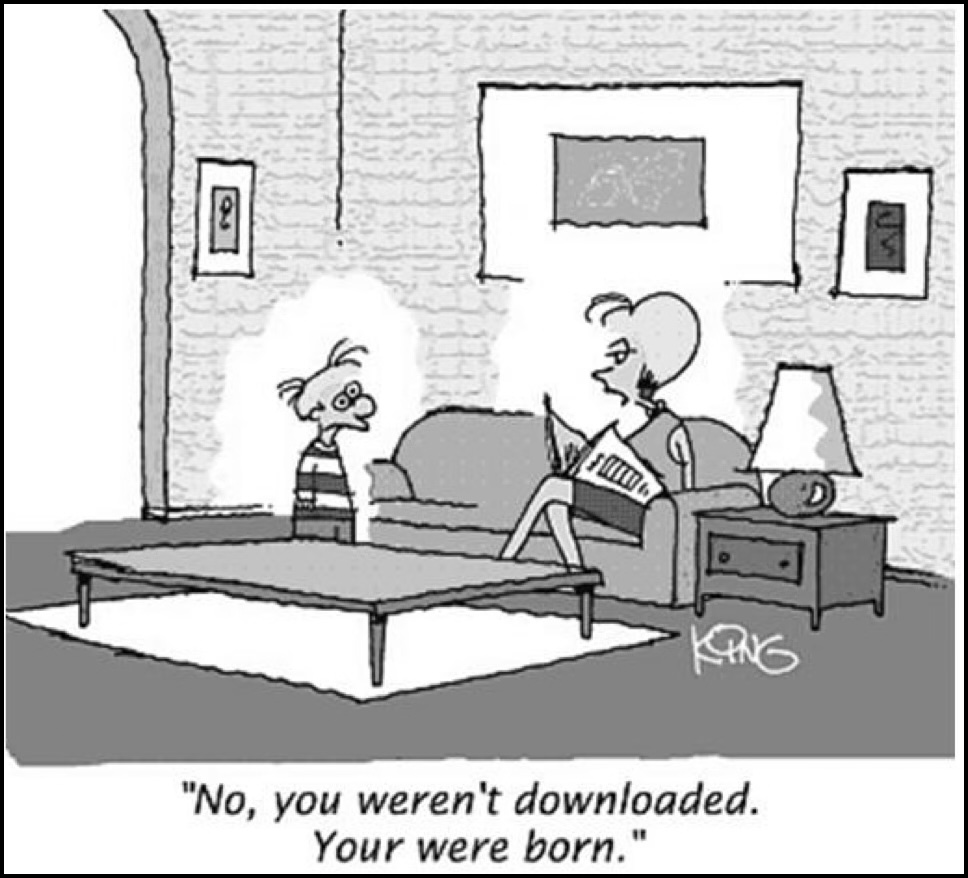
\includegraphics[width=.5\textwidth]{fig1.jpg}
\caption{Uma figura típica}
\label{fig:exampleFig1}
\end{figure}

\begin{figure}[ht]
\centering
\fbox{\includesvg[width=.3\textwidth]{fig3.drawio}}
\caption{Esta figura é um exemplo de uma legenda de figura que ocupa mais de uma linha e 
está justificada, considerando os margens mencionados na Seção~\ref{sec:figs}.}
\label{fig:exampleFig2}
\end{figure}

Em tabelas, tente evitar o uso de fundos coloridos ou sombreado, e evite linhas de contorno grossas, duplicadas ou desnecessárias. Ao relatar dados empíricos, não use mais dígitos decimais do que a precisão e reprodutibilidade dos dados exigem. A legenda da tabela deve ser colocada antes da tabela (veja a Tabela 1) e a fonte utilizada deve ser Helvetica, tamanho 10, em negrito, com 6 pontos de espaço antes e depois de cada legenda.

\begin{table}[ht]
  \centering
  \caption{Variáveis a serem consideradas na avaliação das técnicas de interação}
  \label{tab:exTable1}
  \begin{tabular}{|c|c|c|}
    \hline
    \textbf{Cidade} & \textbf{População} & \textbf{Crescimento} \\
    \hline
    Blumenau & 2.123 & 23,56 \\
    Gaspar & 1.340 & 3,40 \\
    Ilhota & 204 & 1,02 \\
    \hline
  \end{tabular}
\end{table}
    
\section{Images}

Todas as imagens e ilustrações devem ser em preto e branco ou tons de cinza, exceto para os artigos que estarão disponíveis eletronicamente (em CD-ROMs, internet, etc.). A resolução das imagens no papel deve ser de cerca de 600 dpi para imagens em preto e branco, e de 150-300 dpi para imagens em escala de cinza. Não inclua imagens com resolução excessiva, pois elas podem demorar horas para imprimir, sem apresentar nenhuma diferença visível no resultado.

\section{PlantUML}

Tem como usar o PlantUML direto no arquivo Latex, mas precisa incluir a biblioteca \cite{hartmannSpatialPresenceTheory2015}.

% \begin{plantuml}
%   @startuml
%   Alice -> Bob: Hello
%   @enduml
% \end{plantuml}


\section{References}

As citações e referências devem seguir as normas da ABNT. Recomendamos que os nomes dos autores sejam dados entre colchetes, por exemplo: \cite{kolevaPropertiesMixedReality1999}, \cite{toriIntroducaoRealidadeVirtual2020}, \cite{laarniWaysMeasurePresence2015} e \cite{jeraldVRBookHumanCentered2015}.

As referências devem ser listadas utilizando fonte tamanho 12, com 6 pontos de espaço antes de cada referência. A primeira linha de cada referência não deve ser indentada, enquanto as subsequentes devem ser indentadas por 0,5 cm.

\bibliographystyle{sbc}
\bibliography{../UDESC_RV}

\end{document}
